% This is the aspauthor.tex LaTeX file
% Copyright 2010, Astronomical Society of the Pacific Conference Series
%
\documentclass[11pt,twoside]{article}
\usepackage{asp2010}

\resetcounters

\bibliographystyle{asp2010}

\markboth{Shitrasaki {\it et al.}}{Web and Desktop Applications for ALMA}

\begin{document}

\title{Web and Desktop Applications for ALMA Science Verification Data}

\author{Yuji Shirasaki$^1$, 
        Wataru Kawasaki$^1$,
        Satoshi Eguchi$^1$,
        Yutaka Komiya$^1$,
        George Kosugi$^1$,
        Masatoshi Ohishi$^1$,
        and Yoshihiko Mizumoto$^1$}

\affil{$^1$National Astronomical Observatory of Japan,
      2-21-1 Osawa, Mitaka Tokyo, 181-8588, Japan}

\begin{abstract}
%%
ALMA is the largest radio telescope operating in Chile, and 
it is expected to produce 200~TB of data every year. 
%%
Even a data cube obtained for a single source can exceed 1~TB.
%%
It is, therefore, crucial to reduce the size of data transmitted through 
the Internet by doing a cutout of a part of a data cube and/or 
reducing the spatial/frequency resolution before transferring the data. 
%%
To specify the cutout region or required resolution, one needs to overview
whole of the data without transferring the large data cube. 
%%
For this purpose, we developed two applications for quick-looking 
ALMA data cube, ALMA Web QL and Desktop Viewer (Vissage). 
%%
\end{abstract}

\section{Introduction}

The amount of astronomical data has been doubling every 1.5 years 
(Figure~\ref{fig:1}).
%%
On the other hand, the data transmission bandwidth through the Internet 
has not been sufficient for such a rapid increase in the data at all. 
%%
As a result, it is already impossible to retrieve the whole dataset from 
data archives. 
%%

Atacama Large Millimeter/submillimeter Array (ALMA) is the largest radio 
telescope operating in Chile, and it is expected to produce 200~TB of 
data every year. 
%%
Even a data cube obtained for a single source can exceed 1~TB, and it 
is almost impossible to retrieve the whole of the data cube. 
%%
It is, therefore, crucial to reduce the size of data transmitted through 
the Internet, and one needs to cutout a part of a data cube and/or to 
reduce the spatial/frequency resolution before transferring the data. 
%%
To specify the cutout region or required resolution, one needs to overview
the whole of the data without transferring the large data cube. 
%%
For this purpose, we developed two applications for quick-looking ALMA data cube. 
%%
One is a web-based quick look application \citep{O10_adassxxii}, 
which can be used to have a look at integrated images over frequency and 
spatially-integrated spectrum of the data cube; these images can be zoomed 
and centered interactively. 
%%
This web application is written in the HTML5 and the JavaScript, and does 
not require any plug-ins nor add-ons. 
%%
The other is a desktop application, Vissage (VISualisation Software for 
Astronomical Gigantic data cubEs) \citep{P047_adassxxii}. 
%%
Using this application, one can handle data cubes in various modes, such 
as integrated intensity map, 1st / 2nd moment map, Channel map, P-V diagram, 
and so on. 
%%
%% Both of the two applications communicate with the ALMA VO data service, which 
%% is implemented on Table Access Protocol (TAP) specification developed by the 
%% International Virtual Observatory Alliance. 
%%
%% We will demonstrate functionalities of these two applications. 
%%

\begin{figure}
\begin{center}
%%\epsscale{0.3}
%%\plotone{D5_f1.eps}
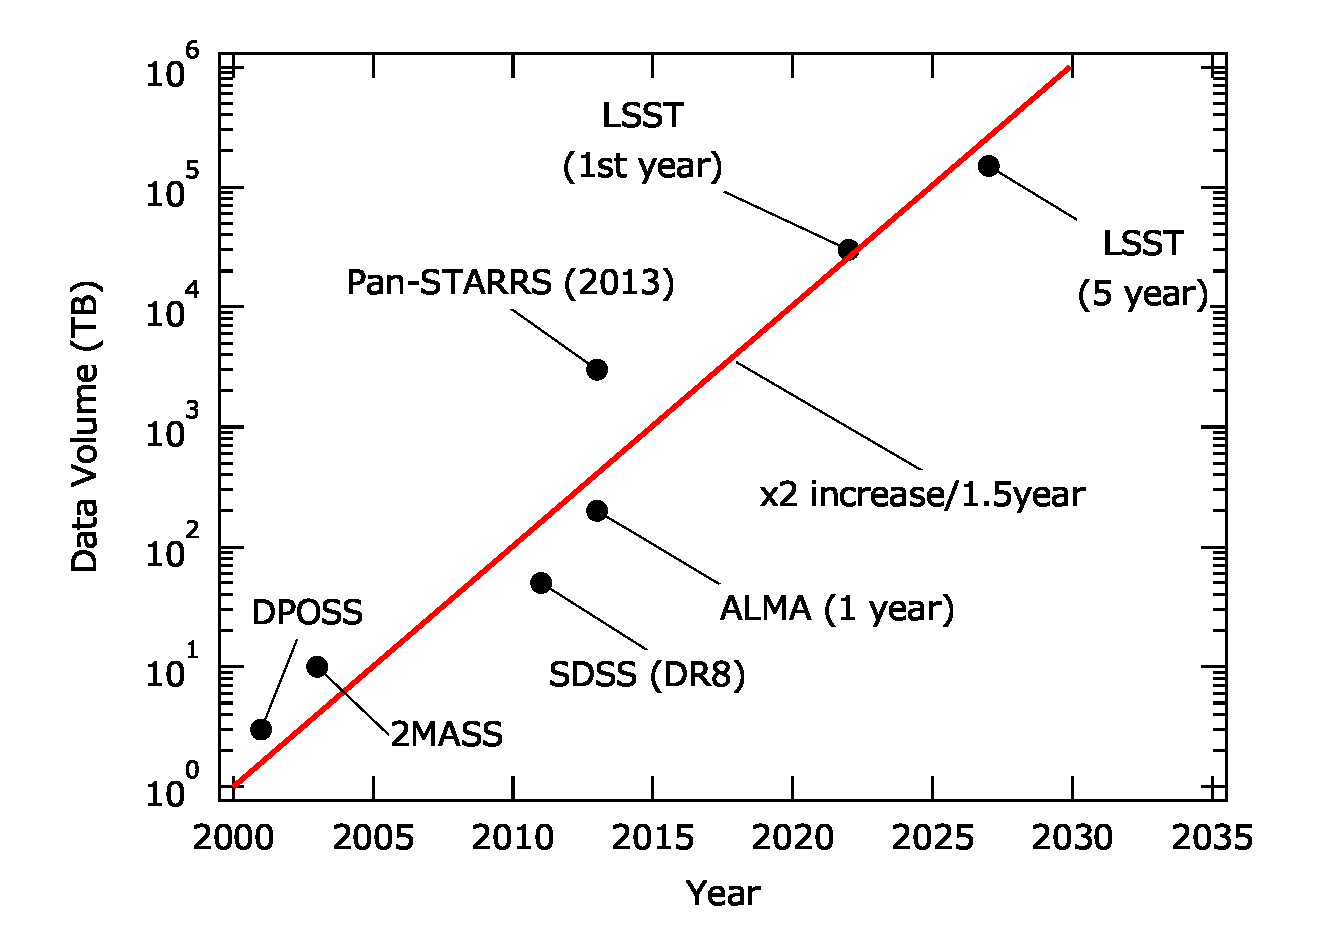
\includegraphics[width = 0.6\textwidth]{D5_f1.eps}
\caption{Data volume by major optical surveys and ALMA.
ALMA: \citet{Lacy_2011},
DPOSS: \protect\url{http://www.astro.caltech.edu/~george/dposs/dposs_pop.html},
2MASS: \citet{Skrutskie_2006},
SDSS: \protect\url{http://www.sdss3.org/dr8/data_access.php},
Pan-STARRS: \protect\url{http://ps1sc.org/Data_Release.shtml},
LSST: \protect\url{http://www.lsst.org/lsst/science/concept_data}.
The line corresponds to a rate of increase twice in 1.5 year.
}
\label{fig:1}
\end{center}
\end{figure}

%%
%%
%%
\section{Architecture}

Figure~\ref{fig:2} shows the architecture of the ALMA-JVO quick look system.
%%
ALMA data are stored on the ''ALMA VO Service'' shown in the right side of 
the figure, and the data search and quick look system, which are used by 
users, are shown in the left side.
%%
Data access interface is implemented base on Table Access Protocol (TAP)
\footnote{\url{http://www.ivoa.net/Documents/TAP/}}
developed by the International Astronomical Observatory Alliance 
(IVOA)~\footnote{\url{http://www.ivoa.net/}}.
%%
By adapting the standard interface, we can easily extend our system to
handle also the data of other VO services.

In order to make this system scalable to the size of ALMA data, we need to
consider how to reduce the size of data transfer between the quick look system
and ALMA VO service.
%%
To reduce the size of data transfer, we have prepared data cubes with a reduced
resolution for each original data cube.
%%
As the amount of information that can be recognized at once on a display 
is limited, it is enough and faster to use an appropriate size of the 
reduced data for a quick look purpose.
%%
The full-resolution data is required when looking at the precise structure
of a small part of the data.
%%
In that case, the part of the data cube can be retrieved by using the
cut-out functionality of the ALMA VO service.

%%
The resolution is reduced by rebinning the original data cube in spatial and
frequency dimensions by factors of (1,2,4,8,16,...)$\times$(1,2,4,8,16,...),
where, for an example, a factor 2$\times$4 means that the data size are 
reduced by 1/2 for each of the two spatial axes ($x$, $y$) and 1/4 for the 
frequency axis ($z$).
%%
The total data size of all the binning data is at most 
$(1 + 1/4 + 1/16 + ...) \times (1 + 1/2 + 1/4 + ...) = 8/3$  of the original data
cube\footnote{Ignoring the size of FITS header}.
%%


\begin{figure}[t]
\begin{center}
%%\epsscale{0.7}
\includegraphics[width = 0.9\textwidth]{D5_f2.eps}
%%\plotone{D5_f2.eps}
\caption{Architecture of the ALMA-JVO Quick Look system}
\label{fig:2}
\end{center}
\end{figure}

%%
%%
%%
\section{Usage Example}

We provides three ways to find ALMA data appropriate for your research.
%%
JVO portal~\footnote{\url{http://jvo.nao.ac.jp/portal}}\citep{Shirasaki_2011} 
provides the easiest way to find the data.
%%
The dataset are classified according to the name of the target~\footnote{We use the 
value of FITS header keyword OBJECT.}, and by just clicking the target name
users are navigated to the data download page.
%%
Thumbnail images for each data cube are also available to see the overview of 
the data.
%%
It is also possible to find the data from JVO Sky 
service~\footnote{\url{http://jvo.nao.ac.jp/portal/jvosky.do}}.
%%

If you are not satisfied with the thumbnail images for selecting the data to download,
try to use the ALMA Web QL by clicking the 'Web QL' button on the download page.
%%
The ALMA Web QL is a simple web-based FITS viewer, which is currently dedicated 
to ALMA data cube.
%%
This web application does not require any plug-ins nor add-ons; just turn on
the JavaScript on your web browser (for most of the case it is set to on by default).
%%
An intensity map integrated over the whole frequency range is shown on the left side
of the page, and a spectrum integrated over the positions displayed on the left
is show on the right side.
%%
Details are described in~\cite{O10_adassxxii}.

If you want to look at the data in more complicated modes, such as 
1st / 2nd moment map, channel map, P-V diagram, and so on, you can download the 
FITS data cube and open it with the ALMA desktop viewer, Vissage.
%%
Vissage is a desktop application developed based on Java, and can be
downloaded at \url{http://jvo.nao.ac.jp/download/Vissage/}.
%%
Details are described in~\cite{P047_adassxxii}.


\begin{figure}[t]
\begin{center}
%%\epsscale{0.7}
\includegraphics[width = 1.0\textwidth]{D5_f3.eps}
%%\plotone{D5_f6.eps}
\caption{Snap shots of each component of the ALMA-JVO Quick Look system}
\label{fig:arch}
\end{center}
\end{figure}


%% \acknowledgements

\bibliography{D5}

\end{document}
